
\chapter{Introduction}

%%% INSERT INTRODUCTION TO THE PAPER HERE %%%


\section{Case}\label{ch:case}
Labelless Media is an ad agency, specialized in making infomercials based on psychology for companies.
This section will describe how Labelless Media currently manages their application system. Moreover, the section will examine the problems that Labelless Media are experiencing with their current way of handling customer leads. A lead is what Labelless Media calls a potential costumer.
\newline \newline \noindent
\textbf{Their current system}\newline
Currently Labelless Media have a simple contact form on their website where the customers are presented with plain text boxes to input their contact information. Their current form can be seen in Figure \ref{fig:CurrentAppForm}.
\newline
\begin{figure}[H]
    \centering
    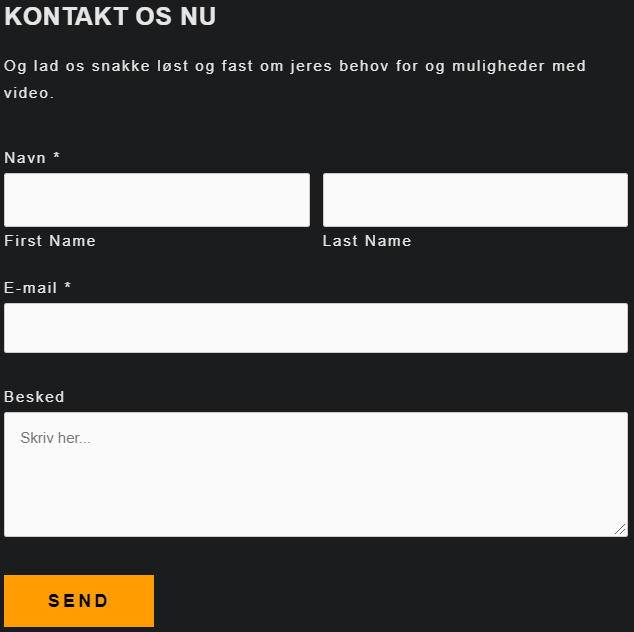
\includegraphics[scale=0.8, clip]{figures/currentApplicationForm.png}
    \caption{The current application form on Labelless Media website}
    \label{fig:CurrentAppForm}
\end{figure}
\noindent
Labelless Media stores their leads in a Excel document. This document is shown in Figure \ref{fig:ExcelDocument}. The Excel document also contains the information about the client, and which product the client want. According to Labelless Media, the way they store their data is poorly organized and confusing. The data is not sorted in any way, so it is difficult for Labelless Media to review the data. 
\begin{figure}[H]
    \centering
    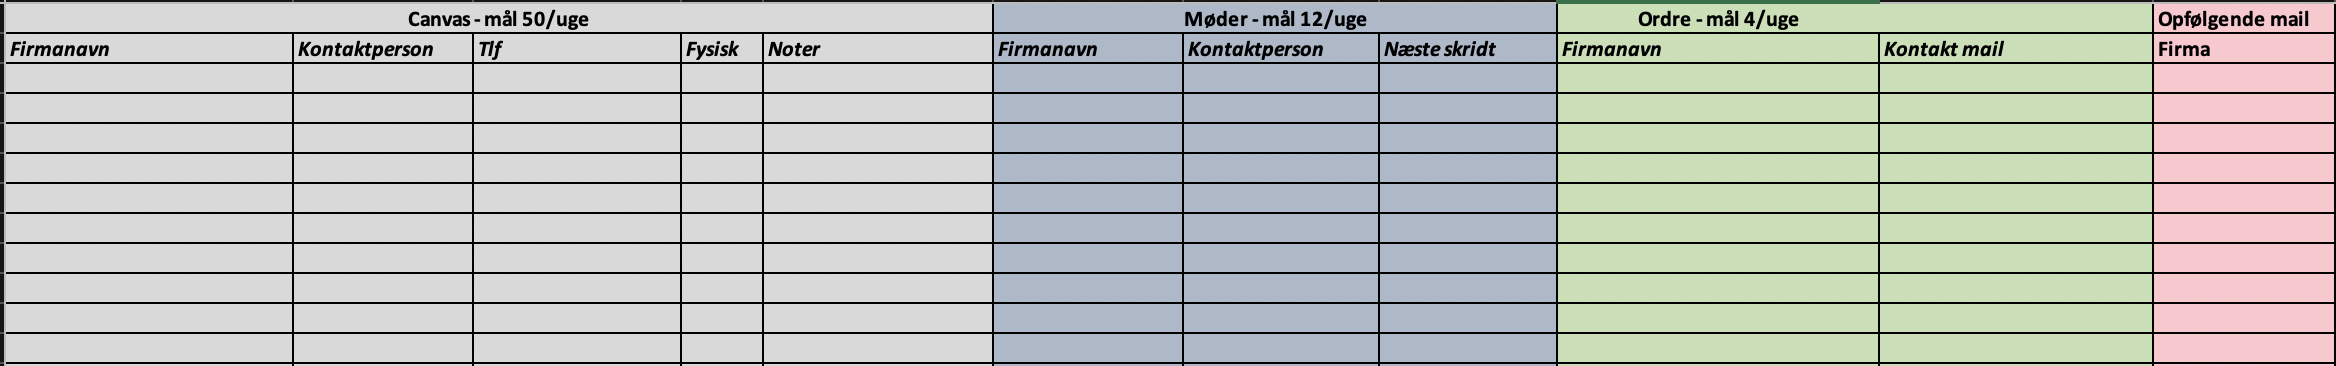
\includegraphics[scale=0.3, clip]{figures/LMExcel.png}
    \caption{The current way Labelless Media stores information about leads in a Excel document.}
    \label{fig:ExcelDocument}
\end{figure}
\noindent
Whenever Labelless Media receives a lead, the lead is inserted into the gray column shown in Figure \ref{fig:ExcelPt1}. In this column, the company name, contact person, phone number and geographical location is saved. 
\begin{figure}[H]
    \centering
    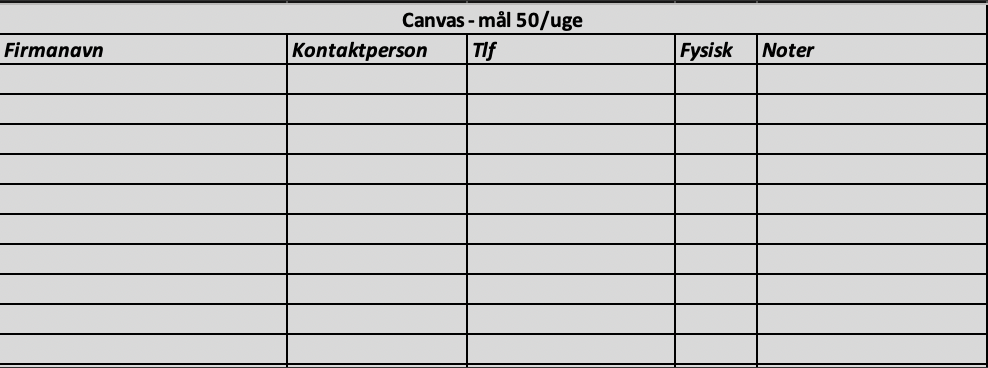
\includegraphics[scale=0.6, clip]{figures/ExcelPt1.png}
    \caption{First part of the Excel document}
    \label{fig:ExcelPt1}
\end{figure}
\noindent
The blue and green columns in Figure \ref{fig:ExcelPt2} indicates if a lead has turned into a meeting or an order. If a lead turns into a meeting, the company name and contact person is listed again. The salesperson also have the opportunity to write down the next step of the process in this column. Whenever a lead turns into an order, the company name and contact email is listed. The red column indicate that the company behind the lead want a consideration period. By inserting companies with consideration period into the red column, Labelless Media makes sure to contact them again.
\begin{figure}[H]
    \centering
    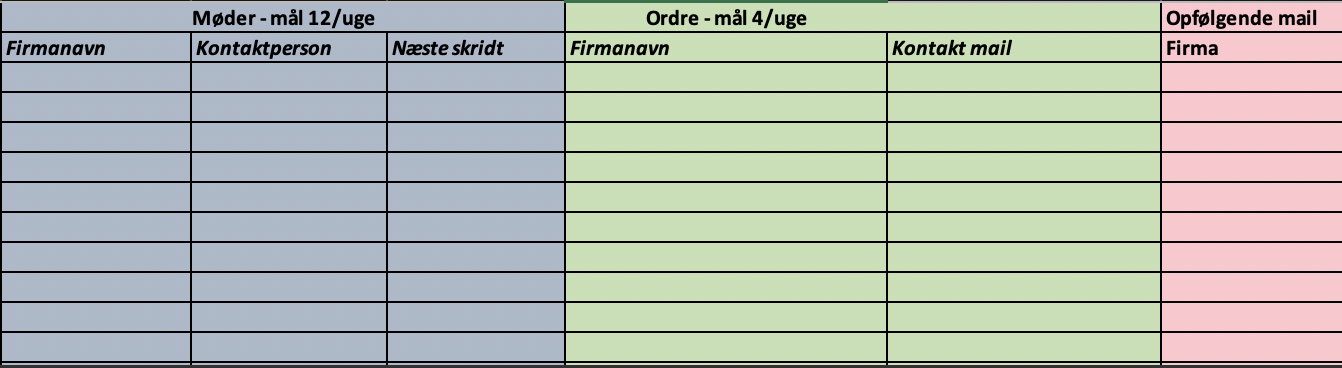
\includegraphics[scale=0.6, clip]{figures/ExcelPt2.png}
    \caption{Second part of the Excel document}
    \label{fig:ExcelPt2}
\end{figure}
\noindent

%%% Problem Statement %%% 
\section{Problem statement}
%Labelless Media's problem concern an absence of a well integrated contact system. Currently companies can contact Labelless Media by mail or phone, which leaves the lead information in an unsorted list across different platforms. It can be a time consuming task to accept the best jobs, and Labelless Media would therefore like to have a system to manage the leads from their clients. 
Labelless Media's main problem is that their current way of handling leads is confusing and poorly organized. All leads ends up in an unsorted excel sheet. Furthermore they find it difficult to pick which leads to follow up on.
%% application form, saving, and sorting system for their customers as well as themselves. %%
\newline \noindent
This results in the following problem statement:
\newline \newline \noindent
\textbf{\textit{The problem is that Labelless Media handles their leads by mail or phone, and they manually evaluate which jobs to accept.}}
\newline \newline \noindent
Thus the paper will investigate how software can improve the way Labelless Media handles their leads by automating the process of evaluation the leads and ranking them by how attractive the job is for Labelless Media.

%%% FACTOR Analysis %%%
\section{Factor analysis}
A factor analysis is made based on the case and problem statement. The purpose of the factor analysis is to specify what the system definition should contain and to get an overview of the system.   
\newline \newline
\begin{tabu} to \textwidth {l X }
   \hline
   Functionality: & 
   The program should be able to consider leads from companies through an interactive gamified contact form. The leads should be evaluated and ranked based on a customizable set of criteria. The users should be able to manage their clients through a client database. \\
   
   & \\
   
   Application domain: & 
   The intended use of the program is to assist the sales personnel in managing client leads. \\
   
   & \\
   
   Conditions: & 
   The program will be used by non IT-educated sales personnel. The development of the system requires access to previous data, to improve and validate the correctness of the system. The contact form must work with the squarespace environment. Furthermore, the interface of the system needs to be compatible with Mac OS. \\
   
   & \\
   
   Technology: & 
   The program will be based on ASP.NET Core and it will run on a Windows 10 or Ubuntu 19.04 server. The system will be developed in C\# using Visual Studio Code and Enterprise. \\
   
   & \\
   
   Objects: & 
   The main objects in the problem domain is the clientele and their leads. \\
   
   & \\
   
   Responsibility: & 
   The system is an administrative tool. The system is responsible for receiving, evaluating, and saving applications from possible customers. The program should consist of a list of contacted and not contacted client leads, a Client database with the possibility to flag and rate clients and the functionality to give an overview of the most promising industries and clients to work with. \\
   
   & \\
   \hline
\end{tabu}


%%% System Definition %%% 
\section{System definition}
A website based system used to rate leads from potential clients based on a set of criteria: Email address provider, yearly turnover, if they have a marketing manager, type of industry and the location of the client.
The system will support marking clients as bad payers.
Furthermore, the priority of the different criteria can be changed by the users of the system and the system itself will automatically update priorities based on previous earnings of client leads. The system will present an overview of contacted and non-contacted clients in the form of two lists. The user is able to sort the two list based on the criteria mentioned earlier. Moreover, the system will be used by a salesman on a Mac.

\section{Summary}
In this first chapter, the case has briefly been described. Labelless Media has shared information about how they currently receive and handle leads, and which drawbacks their current way of working have. On behalf of the information given by Labelless Media, a FACTOR analysis and system definition has been created. These two analysis will serve as a foundation, upon which the system and report will be built. In the following chapter, an analysis of the problem domain will continue to build on the now set foundation.  